\chapter{Specification and design}
\label{ch:specification}

% Choose your own headings.
The design of \textit{Praia Limpa Santa Marta} is focused on creating a platform that meets the specific needs of the Farol de Santa Marta community and its visitors. The following key elements were considered in the design process:


The platform is designed with a user-centric approach, ensuring that it is intuitive and accessible to a diverse audience, including locals, tourists, and environmental activists. Given the varied technical skills of the users, the interface is kept simple yet effective, allowing users of all backgrounds to easily navigate the site and engage with its content.

Considering the international influx of tourists, the platform will support multiple languages, specifically Portuguese and English. This feature is critical for broader accessibility, ensuring that all users, regardless of their native language, can fully engage with the platform. Multilingual support directly addresses the communication needs within the community, facilitating better understanding and participation in conservation activities.

To effectively engage users, the platform includes interactive educational elements such as videos on environmental impact and virtual tours of the beach, which illustrate the effects of littering. These features are designed not only to inform but also to inspire action by demonstrating the importance of conservation efforts in a compelling and immersive way.

Real-time updates are crucial for maintaining community engagement. The platform will provide notifications about upcoming clean-up events and news related to environmental conservation, keeping the community informed and actively involved. This feature supports ongoing participation and fosters a proactive community atmosphere, essential for the success of the conservation initiatives.

\section{System Design}

The system design of the \textit{Praia Limpa Santa Marta} platform is structured to ensure scalability, security, and usability, while meeting the needs of both the local community and visiting tourists. This section outlines the architecture, components, and design considerations that guide the development and deployment of the platform.

\subsection{System Architecture}

The system architecture of \textit{Praia Limpa Santa Marta} is designed to ensure scalability, security, and efficient performance while addressing the needs of the local community and international visitors. The architecture follows a three-tier model, which divides the system into three distinct layers: the presentation layer (frontend), the application layer (backend), and the data layer (database). This separation of concerns facilitates easier maintenance, enhances security, and supports scalability as the project evolves.

\subsection{Presentation Layer (Frontend)}

The presentation layer is responsible for the user interface (UI) and user experience (UX). It is the layer that interacts directly with the users, ensuring that the platform is intuitive, responsive, and accessible across different devices. The key technologies used in this layer include HTML5, CSS3, JavaScript, and Bootstrap.

\begin{itemize}
    \item \textbf{HTML5:} HTML5\cite{html5} is the latest version of the Hypertext Markup Language used to structure content on the web. It provides the semantic foundation for the web pages, ensuring that the content is organized logically and can be easily interpreted by both browsers and search engines. HTML5 supports multimedia elements such as video and audio, and its enhanced features enable the creation of complex web pages without relying heavily on external plugins.

    \item \textbf{CSS3:} CSS3\cite{css3} (Cascading Style Sheets) is used to control the presentation and layout of the web pages. It ensures that the site is visually appealing and responsive, adapting seamlessly to different screen sizes and devices, including desktops, tablets, and smartphones. CSS3 introduces features like animations, transitions, and grid layouts, which enhance the user experience by providing smooth and interactive elements on the page.

    \item \textbf{JavaScript:} JavaScript\cite{javascript} is a scripting language that adds interactivity and dynamic content to the web pages. It allows for the creation of features such as form validation, dynamic content updates, and asynchronous data fetching, which improve the overall user experience by making the site more responsive and engaging.

    \item \textbf{Bootstrap:} Bootstrap\cite{bootstrap} is a popular front-end framework that simplifies the process of designing responsive, mobile-first websites. It provides a collection of pre-designed components, such as navigation bars, buttons, forms, and modals, which can be easily customized and integrated into the site. Bootstrap’s grid system ensures that the layout is consistent across different screen sizes, making it an ideal choice for the \textit{Praia Limpa Santa Marta} project, where simplicity and efficiency are key.
\end{itemize}

\subsection{Application Layer (Backend)}

The application layer, powered by Django\cite{django}, handles the business logic, processes user requests, and manages interactions between the presentation layer and the data layer. This layer is critical for implementing the core functionalities of the platform, such as user authentication, event management, and donation processing.

\begin{itemize}
    \item \textbf{Django:} Django is a high-level Python web framework that encourages rapid development and a clean, pragmatic design. It follows the Model-View-Controller (MVC) architectural pattern, which separates the business logic from the user interface, ensuring that the codebase is modular and easy to maintain.

    Django’s “batteries-included” philosophy means that it comes with many built-in features that are essential for web development, such as an ORM (Object-Relational Mapping) system, authentication mechanisms, and an admin interface. These features allow developers to focus on the unique aspects of the project rather than building common functionalities from scratch.

    \begin{itemize}
        \item \textbf{Object-Relational Mapping (ORM):} Django's ORM provides an abstraction layer that allows developers to interact with the database using Python code instead of writing raw SQL queries. This simplifies database operations such as querying, updating, and deleting records, making the development process faster and less error-prone. The ORM also supports database migrations, which are crucial for managing changes to the database schema over time.

        \item \textbf{Authentication and Authorization:} Django includes a robust authentication system that handles user registration, login, and permissions. This system is essential for managing different types of users, such as volunteers, donors, and administrators, ensuring that each user has access to the appropriate sections of the platform.

        \item \textbf{Admin Interface:} One of Django’s standout features is its built-in admin interface, which provides a user-friendly backend for managing the site’s content and user data. Non-technical staff can use the admin interface to update news articles, manage events, and monitor donations without needing to interact with the underlying code.

        \item \textbf{Security:} Django has several security features built into its core, including protection against SQL injection, cross-site scripting (XSS), cross-site request forgery (CSRF), and clickjacking. These features are crucial for safeguarding user data and ensuring the integrity of the platform, particularly in handling sensitive information such as payment details.
    \end{itemize}
\end{itemize}

\subsection{Data Layer (Database)}

The data layer is responsible for storing and managing the data used by the application, including user information, event details, and transaction records. The \textit{Praia Limpa Santa Marta} platform uses SQLite\cite{sqlite} as its database management system.

\begin{itemize}
    \item \textbf{SQLite:} SQLite is a lightweight, serverless, and self-contained database engine that is fully integrated into the Django framework. It is an excellent choice for small to medium-sized projects due to its simplicity and ease of setup. SQLite stores data in a single file on the server, which reduces the complexity of database management and makes it easy to back up and migrate data.

    Although SQLite is ideal for the early stages of the project, it is designed to scale as the platform grows. As the user base increases and data requirements become more complex, the platform can be migrated to a more robust database system, such as PostgreSQL or MySQL, without requiring significant changes to the application layer. Django's ORM ensures that the transition between different database systems is smooth and minimally disruptive.

    \item \textbf{Data Security and Integrity:} Even though SQLite is lightweight, it still supports transactions and ensures data integrity through the use of the ACID (Atomicity, Consistency, Isolation, Durability) properties. This is particularly important for handling financial transactions and user data, where data loss or corruption cannot be tolerated.
\end{itemize}


\subsection{Key Components}

The system is composed of several key components, each serving a specific function within the platform:

\begin{itemize}
    \item \textbf{User Authentication and Authorization:}
    \begin{itemize}
        \item Django’s authentication system is employed to manage user registration, login, and permissions. This system supports both individual users (e.g., volunteers and donors) and administrative users who manage content and events.
        \item Role-based access control (RBAC) ensures that users have appropriate access based on their roles, preventing unauthorized access to sensitive data or administrative functions.
    \end{itemize}

    \item \textbf{Content Management System (CMS):}
    \begin{itemize}
        \item The built-in Django admin interface functions as the platform's CMS. This interface allows non-technical staff to manage website content, such as news updates, event details, and educational materials.
        \item The CMS is designed to be intuitive, enabling easy updates and content management without requiring deep technical knowledge.
    \end{itemize}

    \item \textbf{Event Management:}
    \begin{itemize}
        \item The platform includes a comprehensive event management module, which allows users to view, register for, and participate in clean-up events. Events are displayed on an interactive map using the Google Maps API, helping users locate nearby activities.
        \item The system supports real-time updates, ensuring that users are informed of any changes to event details, such as time or location.
    \end{itemize}

    \item \textbf{Donation System:}
    \begin{itemize}
        \item The donation system is integrated with Stripe to facilitate secure and seamless financial transactions. Users can contribute to the cause via credit card payments, and the system supports recurring donations.
        \item All financial data is encrypted, and Django’s security features ensure that payment information is processed safely.
    \end{itemize}

    \item \textbf{Multilingual Support:}
    \begin{itemize}
        \item The platform supports multiple languages, including Portuguese and English. This functionality is crucial for ensuring accessibility to both local residents and international tourists.
        \item Language options are provided via a dropdown menu on the website, and all user-facing content is translated to maintain consistency across languages.
    \end{itemize}
\end{itemize}

\subsection{Security Considerations}

Security is a paramount concern in the design of \textit{Praia Limpa Santa Marta}. Several measures are implemented to protect user data and maintain the integrity of the platform:

\begin{itemize}
    \item \textbf{HTTPS:} The entire platform is served over HTTPS, ensuring that data transmitted between the client and server is encrypted and secure.
    \item \textbf{Data Encryption:} Sensitive user information, including passwords and payment details, is encrypted using industry-standard algorithms.
    \item \textbf{Cross-Site Scripting (XSS) and Cross-Site Request Forgery (CSRF) Protection:} Django’s built-in features prevent common web vulnerabilities, such as XSS and CSRF attacks, by sanitizing input and verifying the source of requests.
\end{itemize}

\subsection{Scalability and Performance}

While the initial deployment uses SQLite for simplicity, the system is designed to be scalable:

\begin{itemize}
    \item \textbf{Database Scaling:} As user engagement grows, the system can be transitioned to PostgreSQL or MySQL without significant architectural changes, leveraging Django’s ORM for database migrations.
    \item \textbf{Caching:} Django’s caching framework can be used to store frequently accessed data in memory, reducing the load on the database and improving response times.
\end{itemize}

\subsection{User Experience and Accessibility}

The design of \textit{Praia Limpa Santa Marta} prioritizes user experience and accessibility:

\begin{itemize}
    \item \textbf{Responsive Design:} The platform is fully responsive, ensuring usability across a wide range of devices, from desktops to smartphones.
    \item \textbf{Accessibility:} The platform adheres to accessibility standards (e.g., WCAG 2.1) to ensure that it is usable by people with disabilities, including support for screen readers and keyboard navigation.
\end{itemize}

\section{Testing and Evaluation}

\begin{itemize}
    \item \textbf{Functional Testing:} To ensure all features work as intended across different devices and browsers.
    \item \textbf{Usability Testing:} With real users from the community to gain feedback on the interface and overall user experience.
    \item \textbf{Performance Testing:} To evaluate the responsiveness and stability of the website under various loads.
\end{itemize}

\section{Project Work Plan (10 Weeks)}

\subsection*{Agile Methodology}

The \textit{Praia Limpa Santa Marta} project adopts the Agile methodology, a flexible and iterative approach to software development that is particularly well-suited for projects requiring adaptability, continuous feedback, and stakeholder involvement. Agile emphasizes the delivery of small, incremental releases of the software, allowing for regular assessment and refinement based on user feedback and changing requirements. This approach is advantageous for the following reasons:

\begin{itemize}
    \item \textbf{Flexibility:} Agile allows the project team to respond quickly to changes in requirements, which is crucial for the \textit{Praia Limpa Santa Marta} project, where community needs and environmental conditions may evolve. By breaking the project into smaller iterations or sprints, the team can adjust the scope and priorities as needed without significant disruption.

    \item \textbf{Stakeholder Collaboration:} Agile emphasizes collaboration between the development team and stakeholders, ensuring that the platform aligns with the community’s needs. Regular feedback loops with stakeholders, including local residents, environmental activists, and potential users, help to validate the project's direction and make necessary adjustments early in the development process.

    \item \textbf{Continuous Improvement:} Through iterative development, the project team can continuously improve the platform. Each iteration results in a potentially shippable product increment, which can be tested, reviewed, and refined. This iterative process helps to identify and resolve issues early, leading to higher quality and more reliable software.

    \item \textbf{Risk Mitigation:} By delivering small, functional increments of the platform at regular intervals, the Agile approach mitigates risks associated with project delays, scope changes, and unforeseen challenges. Problems can be detected and addressed promptly, reducing the likelihood of major setbacks.

\end{itemize}
\begin{figure}[h!]
    \centering
    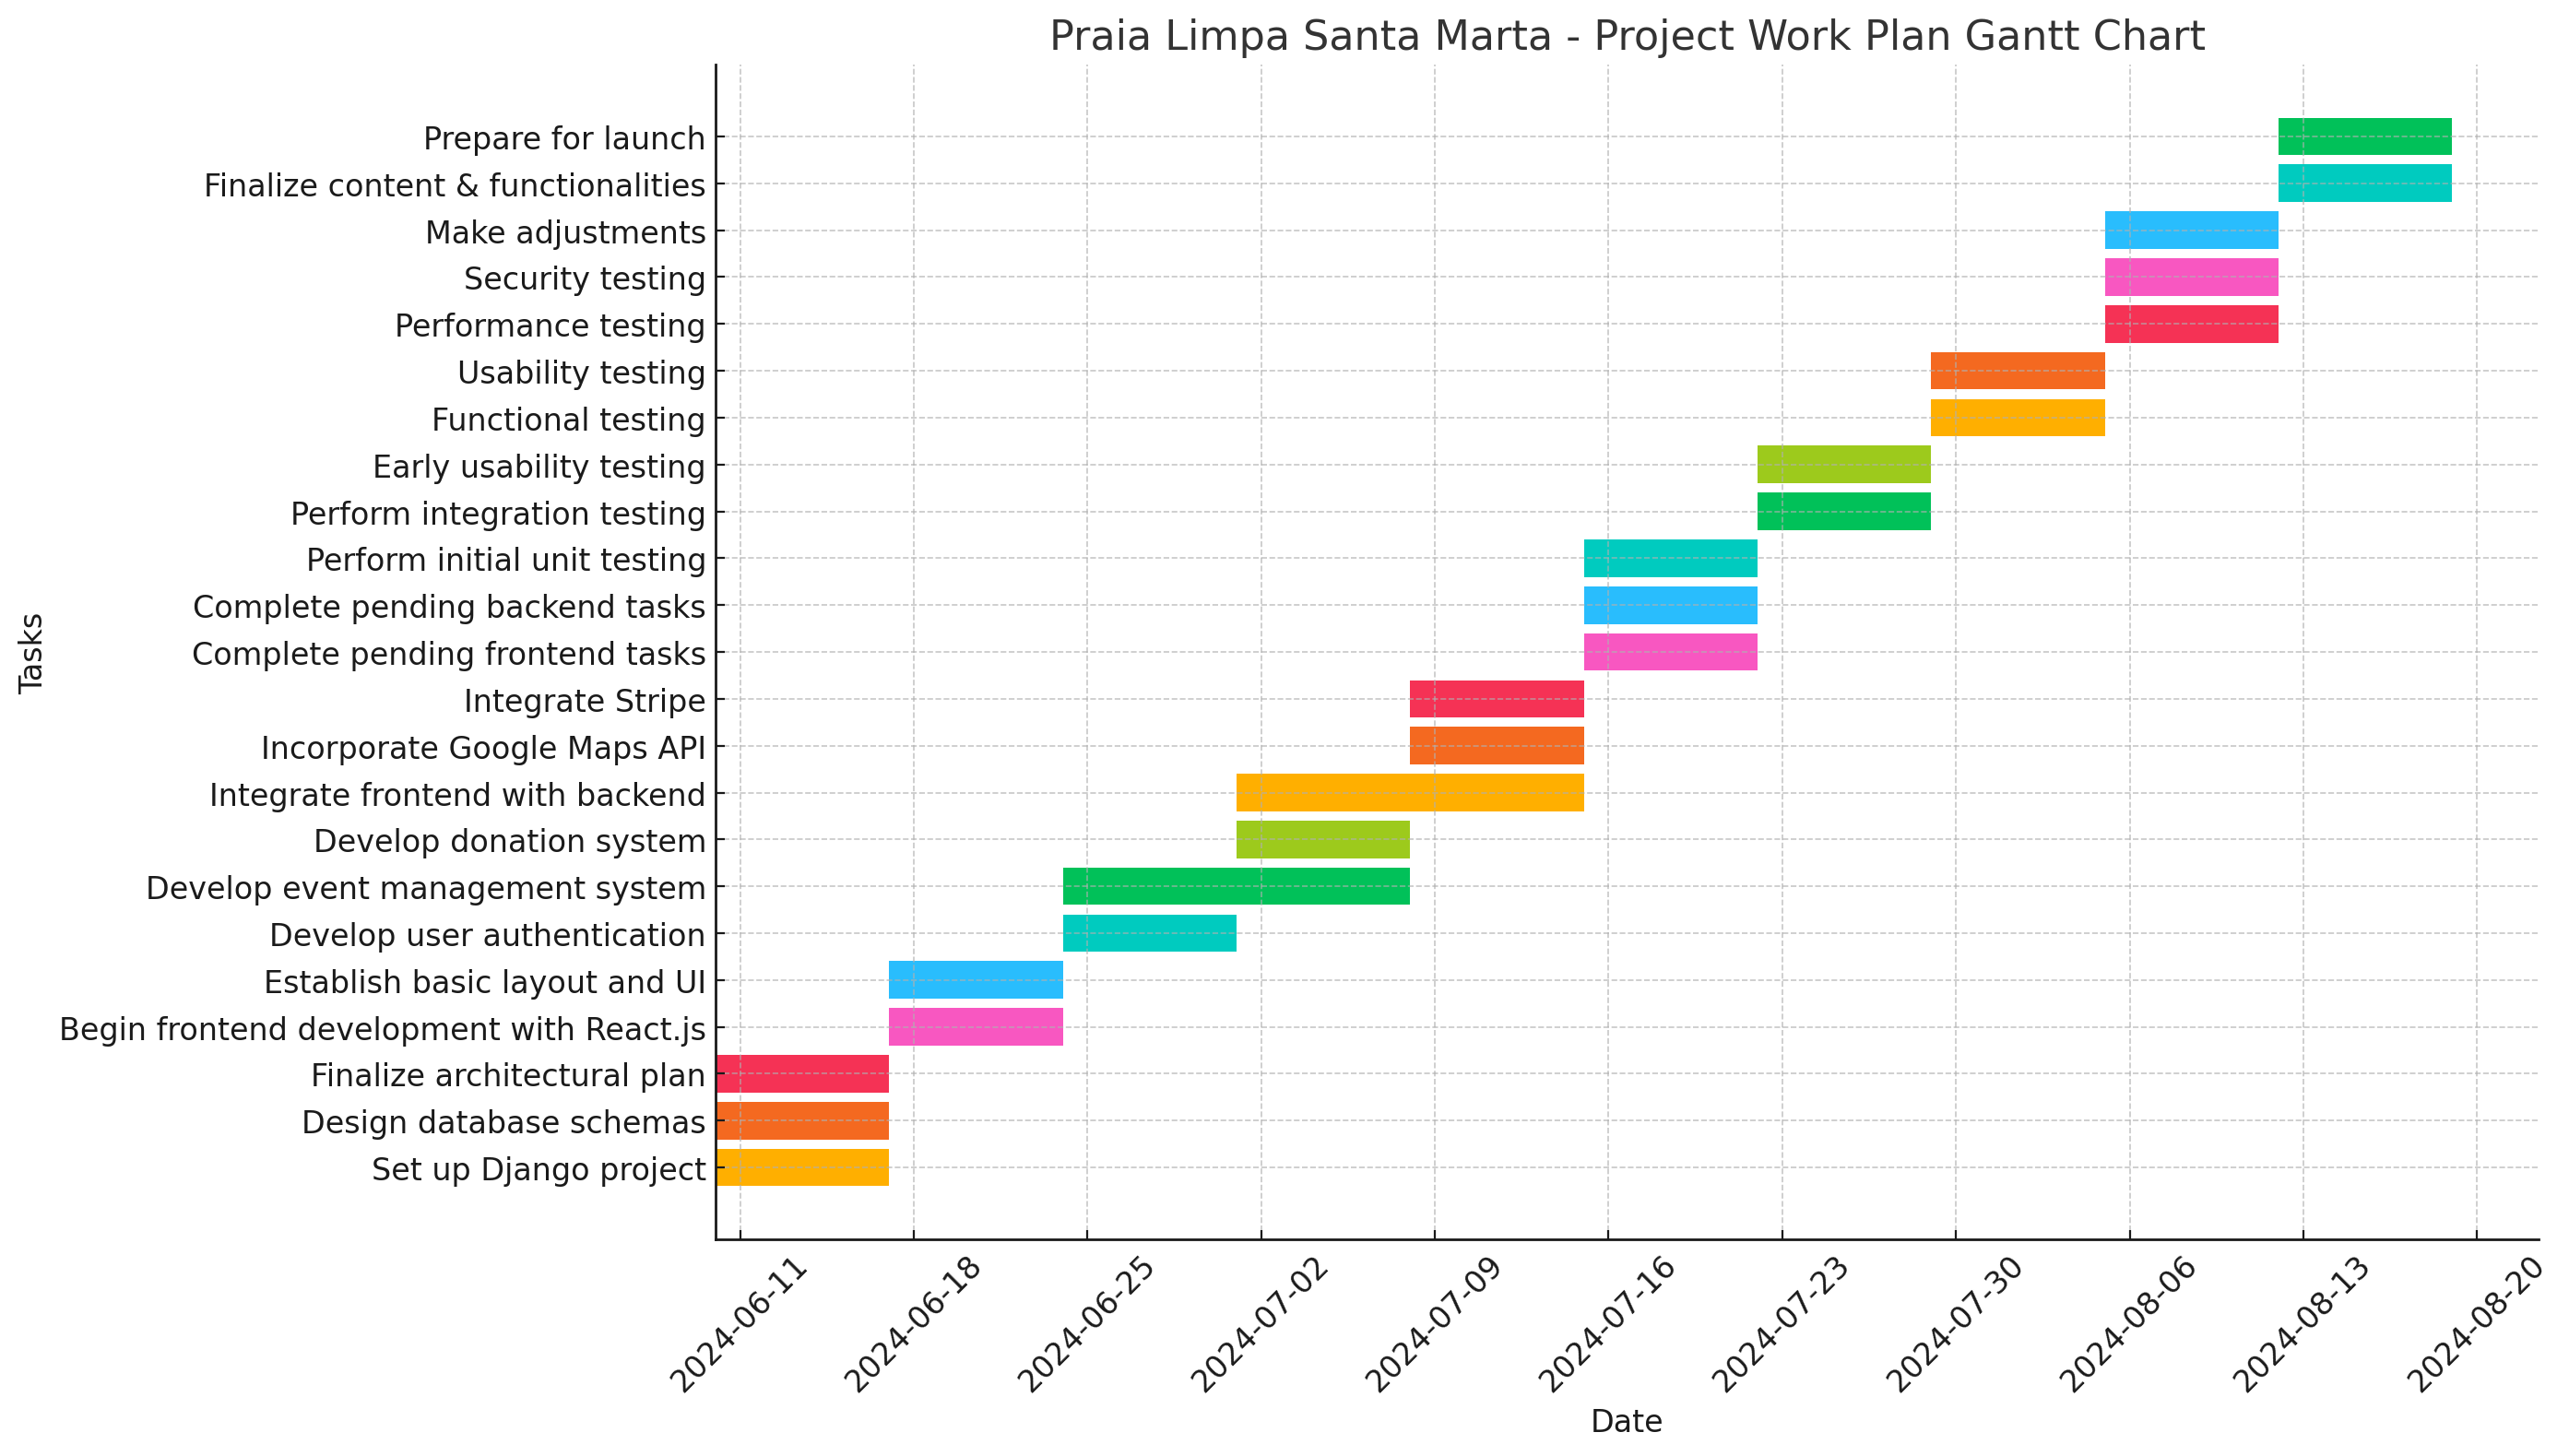
\includegraphics[width=1\textwidth]{images/gantt_chart.png}
    \caption{Project Work Plan}
    \label{fig:work_plan}
\end{figure}

\begin{itemize}
    \item \textbf{Phase 1 (Weeks 1-2):} Requirements Gathering and Initial Design
    \begin{itemize}
        \item Setting up the Django project, designing database schemas, and finalizing the project's architectural plan.
        \item Begin frontend development to establish the basic layout and user interface using HTML, CSS, and Bootstrap.
    \end{itemize}

    \item \textbf{Phase 2 (Weeks 3-5):} Core Development
    \begin{itemize}
        \item Development of the core backend features in Django, including user authentication, event management, and the donation system.
        \item Integration of the frontend with the backend to ensure seamless data flow and user experience.
        \item Begin incorporating external APIs such as Google Maps for event location services and Stripe for donation processing.
    \end{itemize}

    \item \textbf{Phase 3 (Weeks 6-7):} Feature Completion and Initial Testing
    \begin{itemize}
        \item Complete all pending frontend and backend development tasks.
        \item Perform initial unit and integration testing to identify and fix bugs.
        \item Start early usability testing with select community members to gather quick feedback.
    \end{itemize}

    \item \textbf{Phase 4 (Weeks 8-10):} Final Testing, Adjustments, and Launch Preparation
    \begin{itemize}
        \item Comprehensive testing phase, including functional, usability, performance, and security testing.
        \item Make necessary adjustments based on feedback from usability testing and test results.
        \item Finalize content, ensure all functionalities are polished, and prepare for project launch.
    \end{itemize}
\end{itemize}

\section{Kanban Ticketing System}

The development of the \textit{Farol de Santa Marta App} utilized the Kanban methodology\cite{kniberg2010}, a project management approach focused on continuous delivery and flexibility. This allowed the team to manage tasks visually while adapting to evolving requirements. A Kanban board was employed to organize tasks, providing transparency and efficient workflow management.

\subsection{Implementation of Kanban}

The Kanban board, managed using an online tool like monday.com\cite{monday}, was structured with the following columns:

\begin{itemize}
    \item \textbf{Not Started}: Tasks identified but not yet started, including setup, feature development, bug fixes, and documentation.
    \item \textbf{Working on It}: Ongoing tasks that provided visibility and ensured focus on active work.
    \item \textbf{Stuck}: Tasks facing obstacles, highlighting issues early and enabling timely resolution.
    \item \textbf{Done}: Completed tasks, showing progress and ensuring that all reviews and testing phases were passed.
\end{itemize}

\subsection{Application in Development Stages}

\begin{itemize}
    \item \textbf{Setup}: Initial tasks like configuring the Django framework and creating basic models were quickly moved through the board.
    \item \textbf{Feature Development}: Features such as courses, feedback, and the store were broken into smaller tasks and managed systematically through the Kanban system.
    \item \textbf{Bug Fixing}: Bugs and issues were tracked, ensuring timely fixes and project stability.
    \item \textbf{Documentation}: Final tasks related to documentation and deployment were managed through the board, ensuring no step was missed before project completion.
\end{itemize}

\begin{figure}[h]
    \centering
    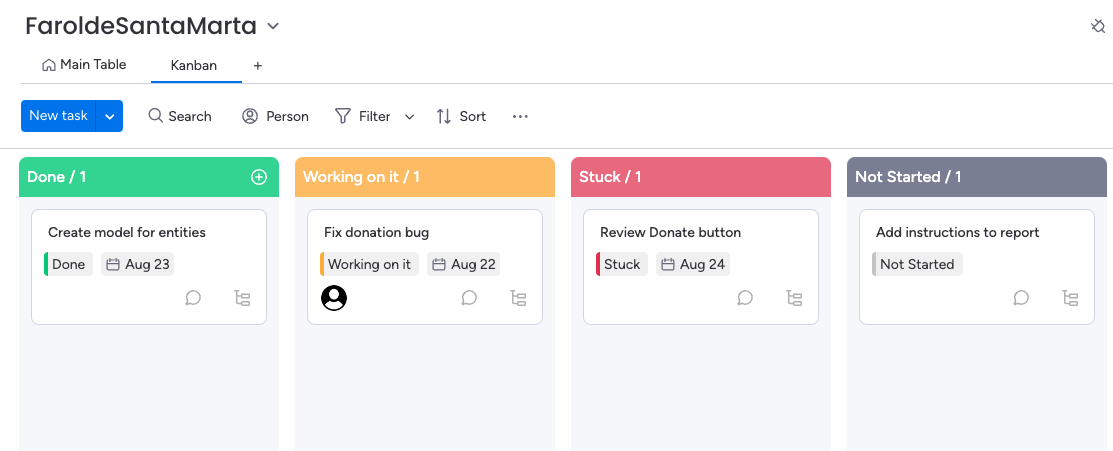
\includegraphics[width=0.8\textwidth]{images/kanban.png}
    \caption{Kanban Board Used in the Farol de Santa Marta App Development}
    \label{fig:kanban}
\end{figure}


%%% Local Variables:
%%% mode: latex
%%% TeX-master: "../../main"
%%% End:
